%===================================== CHAP 4 =================================

\chapter{Implementation}\label{cap_4}

\section{Tools used}

\subsection{ElasticSearch} \label{elasticsearch}
%%JSON abbrevation
ElasticSearch is a tool used in this project for indexing the examples. ElasticSearch is built on top of Apache Lucene(https://lucene.apache.org), which is a information retrieval library, written in Java. Internally in ElasticSearch, data is stored as structured JSON\footnote{JSON - JavaScript Object Notation} documents. The API for communicating with ElasticSearch is a RESTful\footnote{REST - representational state transfer} API using JSON over HTTP. The API can be used for configuring ElasticSearch, building the index and querying it. 
%%Ta med i erfaring seksjon om dette at siden alt dette bruker json og webserveren bruker javascript via node, er alt veldig enkelt og konsistent.

ElasticSearch is built for scalability. This means that it can handle the dataset and interactions growing. This is because it acts as a cluster of many nodes. If the system needs to scale, new nodes can easily be added, and ElasticSearch will distribute resources to the newly added ndoes. However this projects does not need or take advantage of this scaling, and will only be using one node.

When searching in ElasticSearch, there is mainly two ways of doing this. The first one is by using \textit{filter}. The \textit{filter} is utilizing \textit{term} to decide whether a document should be returned or not. Searching with \textit{term} is very similar to how one would use SQL. %Trenger denne forklaring?
Searches can for instance consist of text strings, numbers, ranges or dates, and ElasticSearch will return everything that matches. It also allows for boolean operators and nesting of these. Using a \textit{filter} is very quick and should be used if the relevance of the documents is not important. If relevance score is important then the second option, \textit{query}, should be chosen. If a \textit{query} is combined with a \textit{term}, ElasticSearch is looking for the exact value in its index. A score is then returned based on the documents TF-IDF relevance to the term. See section \label{tfidf} for an explanation of this algorithm.%Burde det referes på denne måten?
If a \textit{match} is used instead, an analysis will be performed, creating a list of terms from the query, and then executing low-level queries for each of the terms. The results are combined to produce the final relevance score. These two methods can also be combined or extended with other methods to customize the search further.


\subsection{NPM and Node.js}
Two of the processes used by this project are written in JavaScript. JavaScript are normally run inside browsers, but by using Node.js\cite{node} the can be executed by a server. Node is an asynchronous event driven framework. By embracing to event loop in this manner, Node avoids thread management and blocking of those. Instead callbacks are pushed on too the event loop and Node runs until there are no more callbacks to perform. This makes Node ideal for simpler and less complex systems, and is why it is chosen for this project.

Node also comes with a packet manager called Node Packet Manager(NPM). NPM allows any Node project, to include libraries and other JavaScript projects published to their \textit{Open Source Registry} \footnote{\url{https://www.npmjs.com/npm/open-source}}. This is done simply by a simple API call to the NPM executable in the terminal. % skriv om hvordan jeg bruker pakkene som tilbys.

Using code from open source libraries saves a lot of time during development while still having full control and overview of the code executed. Because of this a lot of libraries has been used for this project. Examples of libraries used are \textit{sax} for reading the XML file line by line as a stream.  \textit{wtf\_wikipedia} to help out with parsing some of the Wikipedia markup;  \textit{request} to fetch a HTML file from a server with a GET call;  \textit{cheerio} for iterating through an HTML structure while supporting filtering, reading and editing of the HTML. Using libraries results in the system being more modular, which makes it easier to alter during development. This has been highly advantageous for this project, since requirements has been continually changed. 

\section{Pipeline}

Write about the system acting as a pipeline.
Still focus on how this was done.

Should following sections in this capter be sections or subsections?

\section{Source data}


%%vise til XML utsnitt, og skrive litt om det. Skrive på en måte så noen kan dra nytte av det senere
\subsection{XML format}
\begin{figure}[h]
\caption{The XML structure used in the XML dump of Wikipedias database}
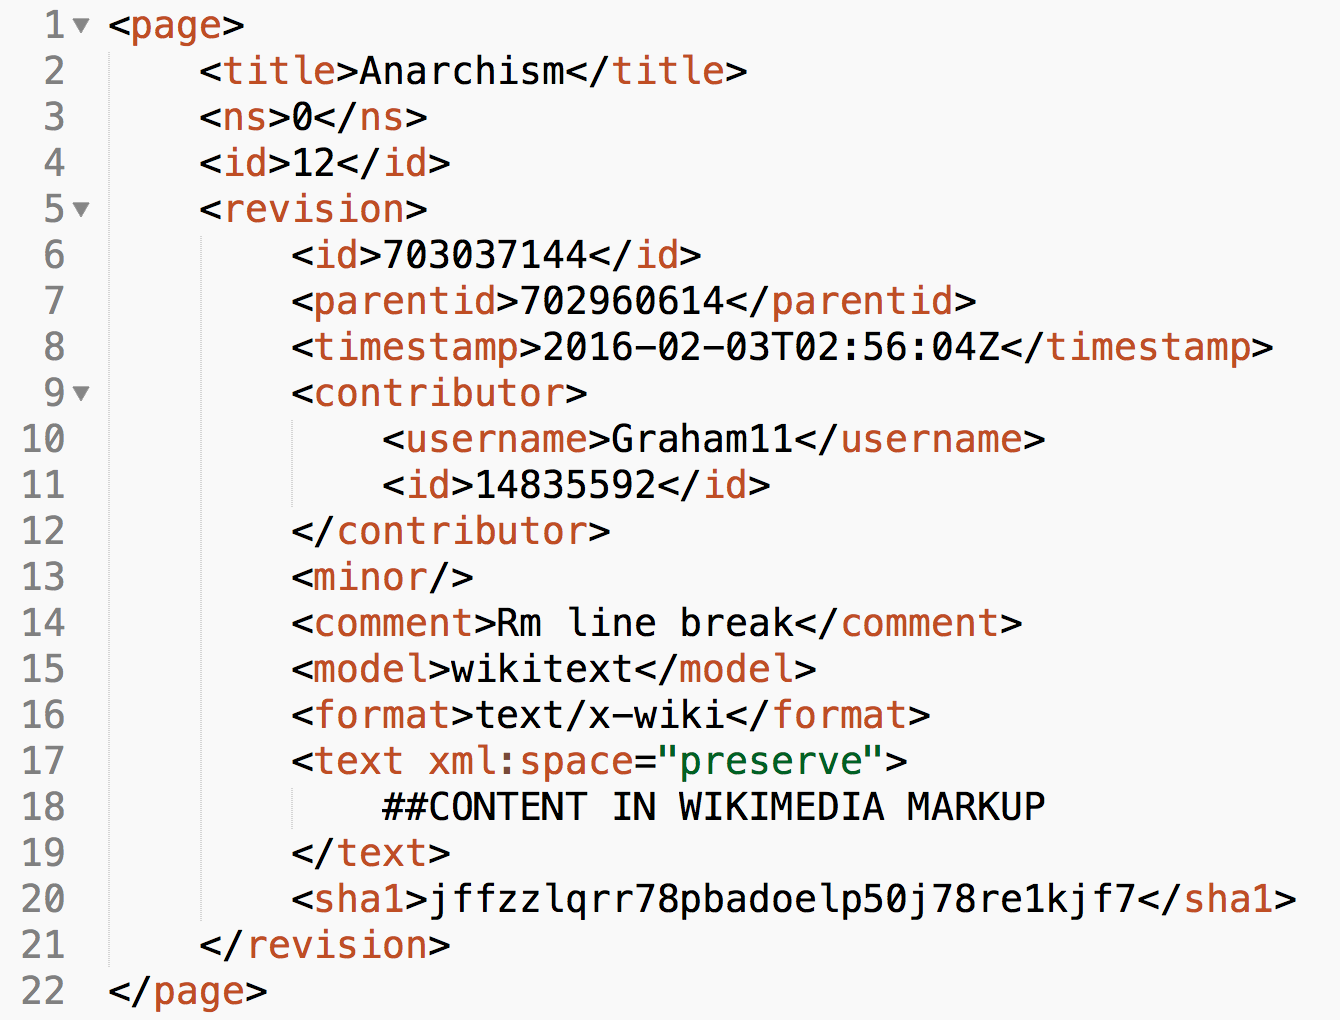
\includegraphics[width=\textwidth]{XMLPage}
\label{fig:xml}
\end{figure}

The source data that is fed into the beginning of the pipeline is on the XML format. \ref{fig:xml} shows how the XML is structured. The file is composed of page elements at the top level with the page tag. Each page element represents an article in Wikipedia. the page has several sub elements, but the most interesting element, is the one with the revision tag. Wikipedia saves several revisions of a page, but in the XML dump used only the newest one is included. It is inside this element that we find the article's content in the form of Wiki markup.


\subsection{XML parsing}


\section{Data retrieval}

%%Parsing XML into relevant data in JSON
\subsection{Wikimedia's markup syntax}


\subsection{Markup parsing}


\section{Data structuring}

%%Inserting the JSON into an sql database
\subsection{Database}

\begin{figure}[h] 
\caption{A simple overview of the database tables and their attributes}
\includegraphics[width=\textwidth]{db_diagram}
\label{fig:db_diagram}
\end{figure}

%% TODO forklare tabellene bedre. Hva de forskjellige termene er i den faktiske wikipedia

Section \ref{custom-pipeline} explains that the source data is fed into the pipeline as a snapshot of Wikipedia at a particular time. The size of the source data is an approximately 50 GB XML-document. Most of this data is not interesting in this project. Therefor the parser excludes most of it before it is structured in the SQL database. 

Figure \ref{fig:db_diagram} displays the tables of the database and the relations between them. If a relevant article is discovered, it is inserted into the \textit{pages} table. The article is found relevant because it contains one or more sections with an example. These sections are then stored in the database with their relation to the article. The categories of the article is also kept, because it will be helpful regarding searching among examples in the finished index.  

The database acts a temporary buffer for the data going into the index. This is helpful because it separates the parsing from the building of the index. This is preferred since the parsing is a very time consuming process, and having it structured in SQL with its meta data helps with showing how successful the parsing was. Most of the meta data is also irrelevant for the index, so only keeping it in the database is beneficial for complexity of the end result.


\section{Indexing data}

Retreviing data fraom the sql database and indexing it.

\section{Searching the data}

Has not been implemented but should maybe be mentioned anyway? Maybe not here?


\cleardoublepage